\qquad A análise de complexidade do Selection Sort, considerando as
diferentes situações de entrada (crescente, decrescente e
randômica), foi realizada manuscrita, com a devida justificativa,
conforme exigido pelo enunciado do trabalho. A digitalização do
material manuscrito deve ser inserida a seguir, substituindo a
imagem de exemplo abaixo.

\begin{figure}[htbp]
    \centering
    % Substitua o arquivo abaixo pela digitalizacao da analise de complexidade manuscrita
    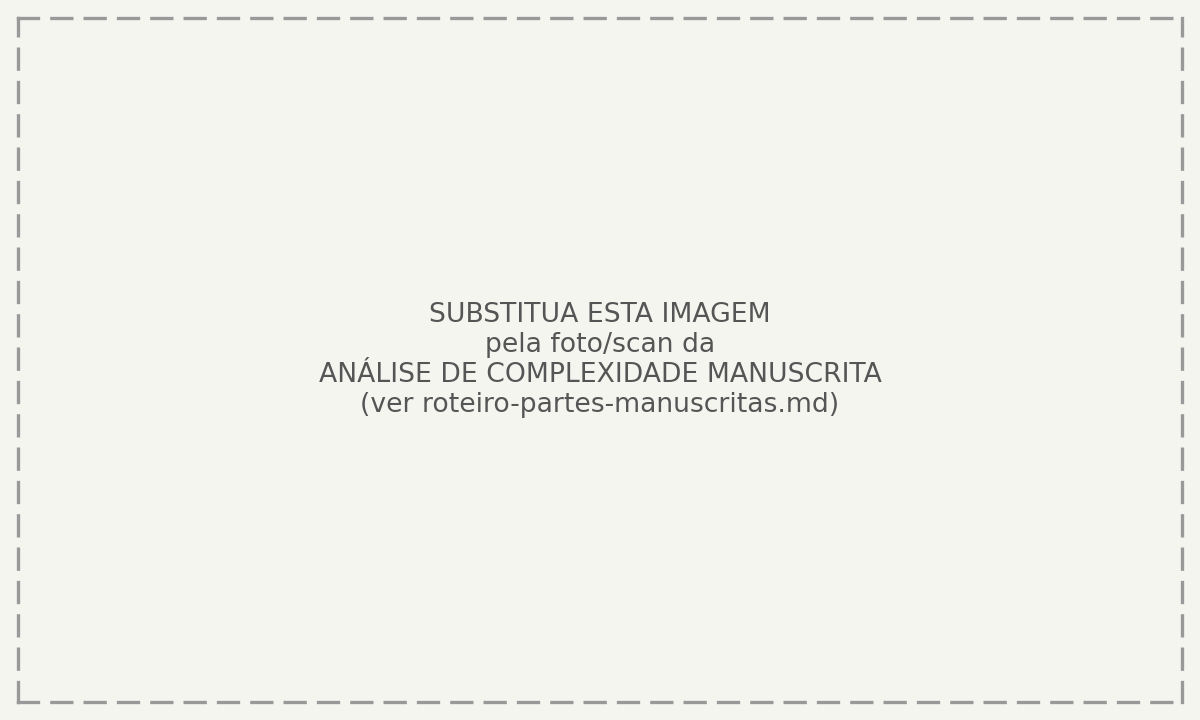
\includegraphics[width=14cm]{Imagens/Selection Sort/analise_complexidade.png}
    \caption{Análise de complexidade manuscrita do algoritmo Selection Sort}
    \label{fig:analise_complexidade_selection}
\end{figure}

\qquad Diferentemente do Insertion Sort e do Bubble Sort, a análise mostra
que o número de comparações do Selection Sort não depende do tipo de
entrada: em todos os casos (melhor, médio e pior) o algoritmo realiza
n(n-1)/2 comparações, resultando em complexidade $\Theta(n^2)$ nos três
cenários. O que varia entre os cenários é apenas o número de trocas
(no máximo n-1), uma quantidade desprezível diante do número de
comparações. Os resultados experimentais apresentados na próxima
seção confirmam essa previsão teórica: os tempos medidos para entradas
crescente, decrescente e randômica são praticamente idênticos entre
si, para um mesmo tamanho de instância.
